\chapter{Scenarios and Projects}
\label{ch:scenariosprojects}
% ##################################################################################################################

\hfill \textbf{Authors:} Andreas Horni, Benjamin Kickh�fer, Dominik Ziemke

\begin{center} 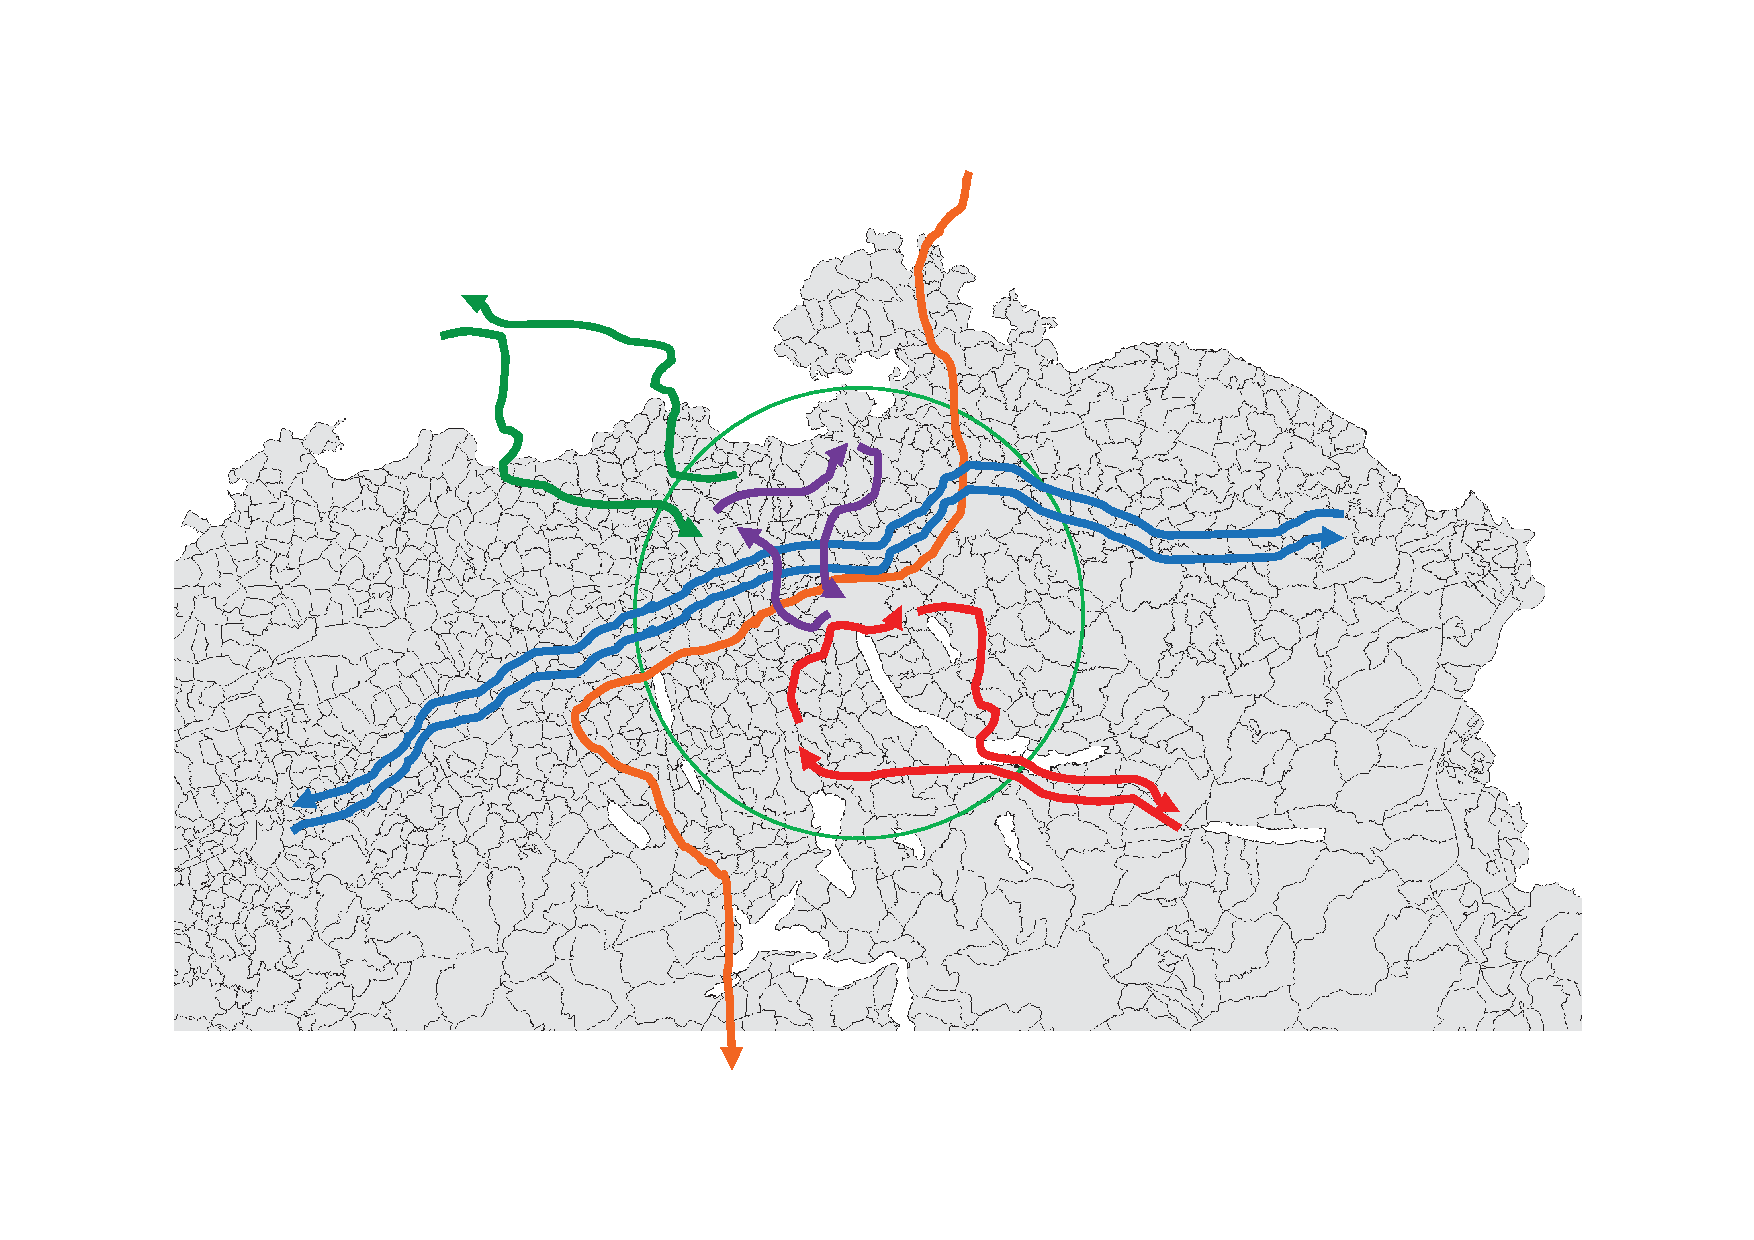
\includegraphics[width=0.7\textwidth, angle=0]{using/figures/zh} \end{center}

% ##################################################################################################################
This chapter summarizes available MATSim scenarios and projects based on MATSim (see also \citet[][]{MATSIM-T-Scenarios_Webpage_2014}). Most scenarios are not public due to privacy issues. However, knowing about the methods used for their creation and problems faced thereby might significantly support the building of new scenarios. 

Scenarios are growing continuously. Here, the latest used version is reported.

Different levels of MATSim involvement are possible. For some regions and projects, MATSim is, for example, only used for traffic assignment whereas for others the complete demand is endogenously handled. Couplings with other forecasting models for transport demand generation have been successfully applied such as the coupling with TASHA for Toronto or the combination of MATSim with the activity-based transport model of Tel Aviv.

% ##################################################################################################################
\section{Scenarios}
This section reports about the study area, demand and supply generation, ...
Utility function is described in Section \ref{sec:utfextensions}.

\ah{Aktuellen Stand von entsprechenden Entwicklern nachfragen/best�tigen lassen.}

%- region description (characteristics, stats, ...)
%- population (popgen, Balmi plug together)
%- facilities
%- network
%- utility function (estimated, how derived)
%- pt (simulated, pseudo pt)
%- modes
%- freight (siehe keynotes Kai)
%- border crossers/boundary effects
%
%data sources
%methods applied
%
%- special problems faced \& solutions found
%
%- simulation quality
%- calibration \& validation (+available data)
%
%- purpose and sponsor/client
%- associated projects -> see Section \ref{sec:projects}
%
%- specialties: parataxis in Gauteng, connections to other sims (Toronto, Tel-Aviv)

% ==================================================================================================================
% ##################################################################################################################
\chapter{Switzerland}
\label{ch:switzerland-scenario}
\hfill \textbf{Author:} Andreas Horni

\editdone{This text has undergone the professional edit. Please no grammatical changes anymore! They are most-probably wrong.}

% ##################################################################################################################
The Switzerland scenario was initially created for the project Westumfahrung \citep[][]{BalmerEtAl_ResRep_bdktzrh_2009} and serves as the base for the very frequently used Zürich scenario (Chapter~\ref{ch:zhscenario}). 

Two main branches can be distinguished. The first, older one is based on a one-to-one translation of the Swiss population census \citep[][]{BfS_VZ_2000}; the second applies approaches from the \gls{ipf} family, reported by \citet[][]{MuellerKAxhausen_TechRep_IVT_2013, Mueller_unpub_LATSIS_2012, Mueller_unpub_ETC_2011, Mueller_unpub_STRC_2011, Mueller_unpub_IATBR_2012} to generate population.

The scenario's study area covered all of Switzerland. Due to administrative borders, no demand and supply data were available for adjoining countries, which, then and now, leads to boundary effects; studies focusing on Swiss border areas are difficult.

The population was derived from the Swiss Census of Population~2000 \citep[][]{BfS_VZ_2000}. The complete Swiss population was modeled, resulting in around 7.5\,million agents. 

This population's home locations were given at hectare level and work locations were specified at municipality level from commuter matrices, a component of the Swiss Census of Population~2000 \citep[][p.35]{BalmerEtAl_ResRep_bdktzrh_2009}. A very good overview, in German, of the population generation, its initial individual demand and activity locations can be found in \citet{MeisterEtAl_SVT_2009}. Further information is given in \citet[][]{CiariEtAl_STRC_2008, MeisterEtAl_WCTRS_2010, BalmerEtAl_ResRep_bdktzrh_2009, BalmerEtAl_ResRep_datapuls_2010, BalmerEtAl_HEUREKA_2008}.

Travel demand was basically taken from the 2000 and 2005 National Travel Surveys \citep[][]{BfS-MZ2005_manual_2006} (Swiss microcensus), although this sample substantially underestimated freight traffic and ignored cross-border traffic of non-Swiss residents. Freight traffic for Switzerland was missing at this time (except Zürich, see next chapter). Cross-border traffic was derived from mode-specific, hourly origin-destination matrices given by \citet[][]{VrticEtAl_ResRep_UVEK_2007}. These were disaggregated to around 600\,000 individual \gls{matsim} plans for the whole country, which contain the cross-border traffic originating \emph{outside} Switzerland. Non-Swiss, cross-border traffic starting in Switzerland was supposed to be negligible. 

The activity location data set, comprising home, work, education, shopping and leisure locations, was also derived from the 2000~Swiss Census of Population and the 2001~Federal Enterprise Census \citep[][]{SwissEnterpriseCensus_manual_2001}, providing hectare level information. Facility generation was described in \citet[][p.33]{BalmerEtAl_ResRep_bdktzrh_2009}.

For car traffic, navigation networks from Teleatlas \citep[][]{MultiNet_Webpage_2010} and \gls{navteq} \citep[][]{Navteq_2011} were available. The most-used network was the planning network derived from from the Swiss National Transport Model \citep[][]{VrticEtAl_BiegerEtAl_2003}.

The public transport simulation network was derived from the National Transport Model of the \gls{uvek}, described by \citet[][]{VrticFroehlich_ResRep_UVEK_2010}. 

The scenario simulated car and public transport; schedules for public transport were given at the municipality level. Fine-granular schedules were not available then, but were in preparation. The modes walk and bike were usually ``\gls{teleported}''. 

Calibration was mainly performed for modal split and distance distributions; utility function values were set accordingly.

For validation, count data on city level, cantonal level and national level \citep[][]{ASTRA_Webpage_2006} were available from various sources, resulting in 600\,links measured for Switzerland. An average working day (Monday to Thursday, excluding public holidays) was used for comparisons in current projects.

% ##################################################################################################################


% ==================================================================================================================
% ##################################################################################################################
\section{Zürich}
\label{sec:zhscenario}
\hfill \textbf{Author:} Andreas Horni

\editdone{This text has undergone the professional edit. Please no grammatical changes anymore! They are most-probably wrong.}

% ##################################################################################################################
The \gls{matsim} team frequently uses the Zürich scenario, based on the Switzerland scenario described above. The Zürich scenario, however, was more detailed; it was enhanced by data available only for the smaller region; \eg traffic light data or freight demand data was only included for Zürich city and the canton. It is under continuous development, calibration and validation and has been applied in numerous projects, serving as a real-world research example.   

\citet{HorniEtAl_TechRep_IVT_2011_a} provided a technical overview of the first scenario branch; \citet[][]{BalmerEtAl_ResRep_bdktzrh_2009} described its generation for the ``Westumfahrung'' project . 

The study area was delineated by a circle, with a 30\,kilometer radius around Bellevue, a central and prominent Zürich location. This delineation led to two versions,  the \emph{Zürich diluted scenario} and the \emph{Zürich cut scenario}. For the first, all agents crossing the study area during the simulated day were considered (Figure~\ref{fig:zurichScenario}), resulting in almost 2\,million agents. For the second, only agents remaining in this area the whole day were modeled. The \emph{Zürich cut scenario} was employed as an experiment in \citet[][]{Hackney_PhDThesis_2009}, but using the \emph{Zürich diluted scenario} for production runs is preferable.

Demand was taken directly from the Swiss model; freight traffic was also added to the Zürich scenario, as follows. Canton Zürich raw freight traffic data was taken from the \gls{kvmzh}, provided by \citet{AMV_Webpage_2011} and documented in \citet[][]{GottardiBuergler_SV_1999}. Zonal level matrices were disaggregated to single \gls{matsim} plans \citep[][]{ShahM_TechRep_IVT_2010}. Matrices for small delivery and heavy trucks were combined into one activity called \emph{freight}. An additional 180\,000 agents were generated for the Zürich region.

For the diluted Zürich scenario, all Swiss facilities, as described above, were used as activity locations. For the diluted scenario, the networks were not thinned out. For  public transport simulation, network and transport schedules were derived from the \gls{kvmzh}. Walk and bike modes were ``teleported''. 

Calibration was mainly done for modal split and distance distributions and utility function values set accordingly.

For validation, count data on city level, cantonal level and national level \citep[][]{ASTRA_Webpage_2006} were available from various sources, resulting in 123\,links measured for the Zürich inner city, delineated by a 12\,kilometer radius around Bellevue. The reduced count analysis radius was applied to reduce boundary effects resulting from demand reduction outside the 30\,kilometer radius study area. An average working day (Monday to Thursday, excluding public holidays) was used for comparison in current scenarios.

Some traffic signal data was available for Zürich city \citep[][]{STAPOZH-DAV_unpub_gtZH_2008}; this was integrated for the Westumfahrung project.
%
\createfigure%
{The diluted Zürich scenario}%
{The diluted Zürich scenario}%
{\label{fig:zurichScenario}}%
{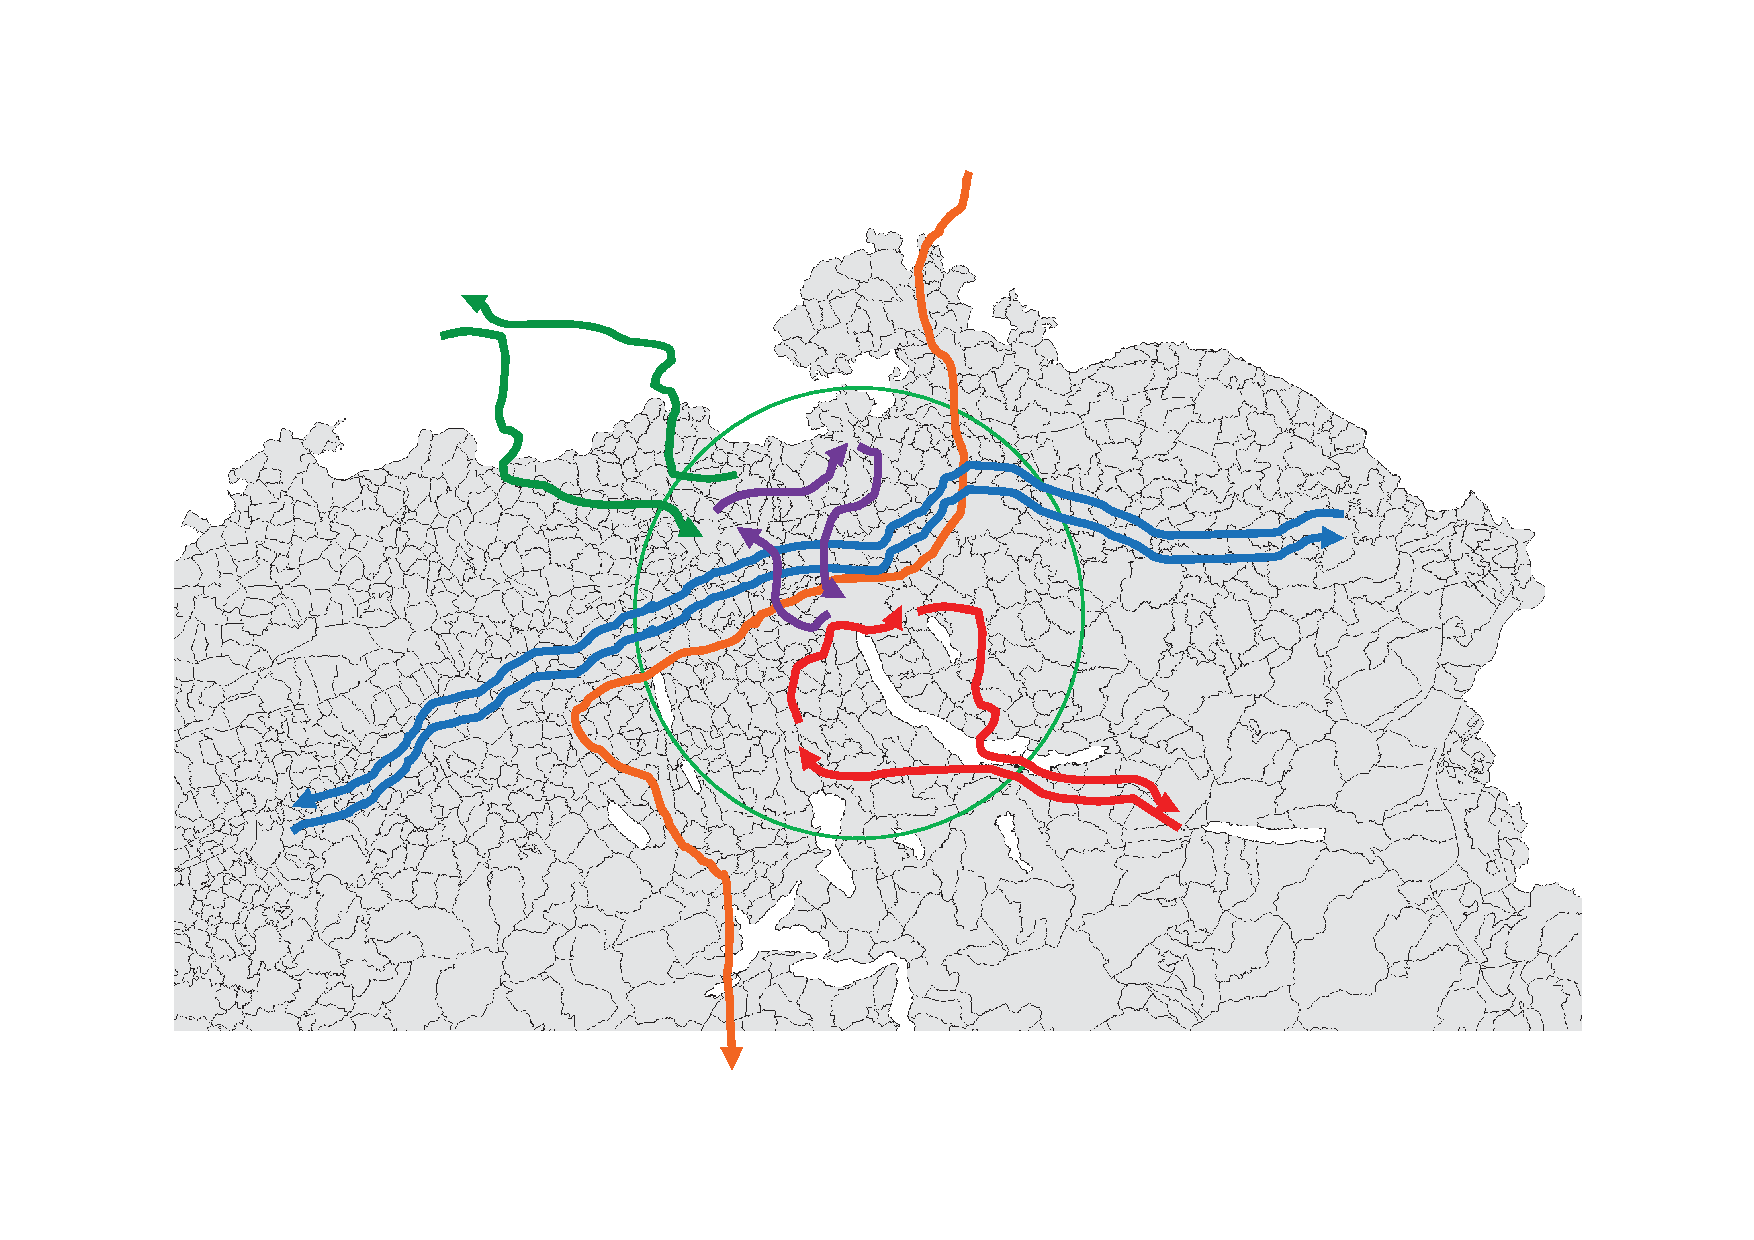
\includegraphics[width=0.99\textwidth, angle=0]{using/figures/zh.pdf}}%
{}

% ##################################################################################################################


% ==================================================================================================================
\subsection{Berlin I: BVG-Scenario \who{Rieser, Neumann}}
\citep[][p.67ff]{Balmer_PhDThesis_2007}

\citep[][Ch 7/8]{Neumann_PhDThesis_2014}

% --------
\paragraph{Associated projects:}

% --------
\paragraph{Study area:}

% --------
\paragraph{Population and demand generation:}

% --------
\paragraph{Activity Locations:}

% --------
\paragraph{Network:}

% --------
\paragraph{Modes:}

% --------
\paragraph{Calibration and validation:}

\ah{Simulation quality, achieved results}

coupling with Visum BVG \\
Marcel: IATBR \\

% ==================================================================================================================
% ##################################################################################################################
\section{Berlin II: CEMDAP-MATSim-Cadyts Scenario}
\label{sec:berlinII}
\hfill \textbf{Author:} Dominik Ziemke

% ##################################################################################################################

As explained in section ?????, transport modeling can be considered as the representation of the interaction of transport demand (i.e. people and goods being transported) and transport supply (i.e. transport infrastructure and services) in the transport system. Depending on the application of innovative strategy modules (see section ?????), MATSim accounts for the adaption of transport demand to transport supply \citep{Balmer2007phd}. It is, therefore, crucial to distinguish choice dimensions, which may be adapted during the modeling process (via the application of innovative strategy modules, see section....) and choice dimension whose initial properties are assumed to be correct (e.g. mode shares have to be initially correct in a scenario where the choice of transport modes is not modeled). In the latter case, it is important that respective properties of the transport demand are correct at the start of the simulation (see section Data Requirements - Demand???).

In order to model these properties of the initial demand correctly, suitable data are needed. A widely utilized source of such data are travel diaries, which contain sequences of departure times, mode choice decisions, and activity locations.
%A disadvantage of using trip diaries is, however, that all information that is taken from the diaries is by definition not sensitive to policy measures. Also, trip diaries are normally only available for a very small fraction of the population. Another drawback is that, in Germany and the U.S. (and many other parts of the world), the geo-coding of the activity location is considered sensitive information under privacy legislation, and thus increasingly difficult to obtain (cite ZiemkeNagelBhat2015).
Many contents of this data source, in particular information concerning locations, are, however, in many parts of the world (e.g. in Germany and the United States) considered sensitive in terms of data privacy legislation and thus increasingly difficult to obtain and to process \citep{ ZiemkeNagelBhat2015IntegratingCemdapMatsimTransferabilityTRB}.

The \textit{Berlin II scenario} (also referred to as the \textit{CEMDAP-MATSim-Cadyts scenario} according to applied models in its setup) is the outcome of an alternative approach that relies exclusively on input data that are freely available and easy to obtain. The starting point for the Berlin II scenario are publicly available commuting matrices which contain home and work places of socially-secured workers on the municipality level. Based on this information, it is possible to model morning and evening commuting peaks.

In order to obtain a demand representation of the full population, two further major modeling steps are required. First, in cases (like in the Berlin case, see below), where the spatial resolution of the commuter matrix is quite coarse, a method to attain origin-destination information at a higher resolution is needed. Second, there needs to be a procedure to model secondary activities, i.e. all other activities that go beyond home and work activities.

The necessity of the first step becomes obvious when looking at the German case, where, for instance, all of the city of Berlin, with 3.4 million inhabitants, is represented by exactly one zone \citep{BA2010Pendlerstatistik}. In the U.S., commuting matrices are typically available only at a county-to-county level. Since such location-aggregation-based matrices may become the rule rather than the exception in privacy-sensitive societies, a (generalizable) method to attain origin-destination information at a higher resolution is needed \citep{ ZiemkeNagelBhat2015IntegratingCemdapMatsimTransferabilityTRB}. The standard solution would be to estimate an activity location choice model. This, however, is difficult if no trip data to estimate the model is available. OD matrix estimation studies \citep{ZuylenWillumsenMatrix-from-cnts} suggest that traffic counts may be used to make an initially rough OD matrix more appropriate for a region. As MATSim is not based on OD flows (see section ????), but on full daily plans, the issue becomes whether there is a procedure to update these initial full daily plans using traffic counts. In the approach to create the Berlin II scenario, a procedure proposed by Flötteröd et al. \citep{FloetteroedBierlaireNagel2010Bayesian} and implemented in the software Cadyts (Calibration of Dynamic Traffic Simulations \citep{Floetteroed2010Manual110}) is applied for this task. Specifically, random draws of possible home and work locations within the home or work municipality given by the commuter matrix are taken. Various MATSim plans each containing one pair of home and work locations are created for each agent. Then, the Cadyts calibration procedure is applied within the iterative MATSim simulation to select those plans, and thus also those locations, which appear more plausible with regard to given traffic counts.

As stated above, however, full daily plans (as opposed to mere home-work-home comuting patterns) are needed. Therefore, the second aforementioned additional modeling step, the modeling of secondary activities for each individual in the region, needs to be addressed. For the Berlin II scenario, the Comprehensive Econometric Microsimulator for Daily Activity-Travel Patterns \citep{BhatEtAl2008CEMDAPUserManual} is used to generate initial complete daily plans for each individual. One the one hand, however, no CEMDAP parameter set is available for Berlin. On the other hand and more importantly, one major goal of the study creating the Berlin II scenario was to show is generalizability \citep{ ZiemkeNagelBhat2015IntegratingCemdapMatsimTransferabilityTRB}. So, the model parameters of CEMDAP estimated for the Los Angeles region (the estimation context) are retained, and then used to generate the initial plans for individuals in Berlin (the application context in the current paper) based on Berlin demographic data.

To sum up, home and work municipalities are taken from the commuter matrix. Within these municipalities, a set of (more precisely spatially defined) potential home and work locations are randomly chosen for each agent. Full daily plans incorporating the various potential locations of each agent are generated with CEMDAP based on a parameter set from another region and local demographic data.

Then, the Cadyts calibration procedure is used to select those initial full daily plans that are most consistent with Berlin traffic count data. In other studies, Cadyts has already been applied to update route choice predictions, both for car \citep{FloetteroedChenEtAl2011BehavioralCalibAndAna} and for public transit \citep{MoyoNagel2013ptNetCalibrationABMTPO}. However, it has not been used to update full daily activity-travel plans, as it has been done in the procedure that created the Berlin II scenario. 

As a result, the Berlin II scenario, is an activity-plan-based MATSim transport model for Berlin that is exclusively based on freely or easily available data. If a commuter matrix, some basic demographics of the population, and traffic counts (or theoretically another suitable data source to run the calibration procedure on) are available for a particular regional context, the approach used to create the Berlin II scenario can be transfered to this context. In fact, the Berlin II scenario itself has to be seen as a \textit{transferred model} because the initial plans generated by CEMDAP are based on parameter estimates from another geographic region (namely the Los Angeles area).

Through a validation based on the Berlin 2008 SrV \textit{System repräsentativer Verkehrserhebungen}, an extensive, regularly conducted travel survey, the quality of the created transport demand representation has been successfully tested. So far, the Berlin II scenario exists for a 1\%{} and a 10\%{} population sample of all persons, i.e. also non socially-secured workers and also non-working people, aged 18 and above for the study region. Currently, only motorized traffic is considered. Stability tests, showing that agents' daily plans keep being chosen when the Cadyts calibration functionality is switched of, have been successfully carried out. This can be seen as a clear indication that the scenario is applicable for policy studies in a meaningful way.

Further improvements like the addition of public transport and a more realistic representation of the population are planned. Moreover, similar approaches of integrating activity-travel pattern generators (e.g. the FEATHERS model, cite?????) with MATSim as a transport simulation are planned.

\ah{NOTES: to be removed:
AN: Szenario entstand aus einer Arbeit zur Nachfragegenerierung. Würde also auch in einen conceptual part passen, anderer Ansatz als die meisten anderen Szenarien ("datensparsam"), Integration von CEMDAP (Modell zur Aktivitätenkettenerzeugung)

Auch link auf Cadyts.

Aktivitätenkettenerzeugung: ähnlich zu Tel Aviv Modell

FEATHERS am Beginn -> Vortrag Wiepersdorf
}

% ##################################################################################################################

% ==================================================================================================================
\subsection{Singapore (Author: ...)}
The Singapore scenario is build at the Future Cities Laboratory in Singapore embedded in the Singapore National Research Foundation initiative CREATE (Campus for Excellence and Technological Enterprise). The scenario is detailed by \citet[][]{ErathEtAl_TechRep_FCL_forth, Erath_unpub_UniSeoul_2011}.

% --------
\paragraph{Associated projects:} 
The scenario is built for the MATSim Singapore project presented in Section \ref{sec:singaporeproject}.

% --------
\paragraph{Study area:} 
The scenario covers the whole republic of Singapore with its approximately 5 million inhabitants.

% --------
\paragraph{Population and demand generation:} 
For population generation an IPF-approach is adopted. A full-population census is not available for Singapore. Demand is derived from a national travel diary survey (Household Interview Travel Survey) reported by \citet[][]{Choi_JOUR_2010} and containing about 11'000 households in Singapore. Home and work locations are assigned by employing a gravity-model-like approach. Freight trips and non-permanent resident inhabitants' trips are generated from origin destination matrices provided by the Singapore Land Transport Authority (LTA).

% --------
\paragraph{Activity Locations:} 
Activity locations are defined at a single building level. Various sources as described in Section 4.1 of \citet[][]{ErathEtAl_TechRep_FCL_forth} have been merged. Workplace capacities are estimated by \citet[][]{OrdonezErath_TRR_2013}. This is required for assigning the fixed activity locations to the agents.

% --------
\paragraph{Network:} 
For the Singapore model both a planning network (provided by LTA) and a Navteq navigation network are readily available. These two networks are combined for the Singapore scenario by a semi-automatic map-matching algorithm. Public transport routes are matched to the network by another map-matching algorithm presented by \citet[][]{Ordonez_HKSTS_2011, Ordonez_Webpage_2011_4}. This enables interaction between public transport and individual traffic.

% --------
\paragraph{Modes:} 
The scenario simulates car and public transport. The modes walk and bike are ``teleported''. Public transport schedules were derived from General Transit Feed Specification (GTFS) created by Google.

% --------
\paragraph{Calibration and validation:}
For validation road count data on an hourly base are available for 200 stations in Singapore.

% --------
\paragraph{Simulation quality and achieved results:}

% --------
\paragraph{Miscellaneous, important to mention:}
Traffic lights are not yet included in the model due to missing data on signal schedules.

% ==================================================================================================================
% ##################################################################################################################
\subsection{Munich, Germany}
\label{ch:scenarios:munich}
\hfill \textbf{Author:} Benjamin Kickh\"ofer

The \acrshort{matsim} scenario for the Munich metropolitan area was set up during the year 2010.%
%
\footnote{
%
The most detailed descriptions of the scenario can be found in \citet{KickhoeferEtAl_VanoutriveVerhetsel_2013} and \citet{Kickhoefer_PhDThesis_2014}.
%
}
%
The main goal was, and still is, the simulation of local air pollutant and global greenhouse gas emissions, and how their levels change with respect to different policy measures -- on aggregated and spatially disaggregated level. The scenario was therefore used for the development and testing of the \gls{emt} (see Ch.~\ref{ch:emissions}).

Network information from \acrshort{visum} was converted into \acrshort{matsim} format, resulting in a network of 17'888 nodes and 41'942 links.
%
This transport supply was then linked to travel demand from different sources: an activity-based demand for inner-urban traffic from survey data was created based on "Mobility in Germany" \citep[MiD 2002,][]{FollmerEtAl_TechRep_infasDIW_2004}. This part of the synthetic population consists of roughly 1.4m individuals with detailed vehicle information for every household.
%
Commuter and reverse commuter were modeled based on data provided by the German Federal Employment Office \citep{BoehmeEigenhueller_TechRep_IAB_2006}. This part of the population consists of roughly 0.5m individuals from which 0.3m commute to Munich for work. The remaining individuals live in Munich and commute to their workplace in the surroundings of Munich.
%
Freight traffic was also introduced into the model by using data from the German Ministry for Transport \citep{ITBBVU_TechRep_2007}. This part of the population consists of roughly 0.15m freight vehicles who perform one single commercial trip per day.

The scenario has so far been used for several case studies:
%
\citet{HuelsmannEtAl_LAS_2011} used a single street corridor of the scenario to validate simulated travel times and emission levels against actual data obtained from a test vehicle.
%
\citet{KickhoeferEtAl_VanoutriveVerhetsel_2013} investigate the relationship between the price elasticities of car travel demand and those of air pollutant emissions.
%
\citet{HuelsmannEtAl_GerikeEtAl_2013} identify areas with high air pollution concentration in the city. They define these areas as 'hotspots' since the \gls{eu} limits for \gls{no2} are exceeded. The authors then incrementally raise the toll levels for passing the hotspots until they disappear in order to estimate the true avoidance costs of the \gls{eu} threshold values.
%
\citet{KickhoeferEtAl_NSE_2013} derive time-dependent vehicle-specific first-best air pollution tolls in order to create a benchmark for the evaluation of real-world policies.
%
\citet{KickhoeferKern_MobilTUM_2014} go a step beyond and calculate time-dependent vehicle-specific air pollution exposure tolls in order to correct the toll levels by \citet{KickhoeferEtAl_NSE_2013} for the number of affected individuals.



% ##################################################################################################################

% ==================================================================================================================
\subsection{City of Sioux Falls (South Dakota)}

Often used test scenario \citep[][]{BarGera_TNTP_Webpage_2013}. Not aimed at replicating the real City of Sioux Falls, South Dakota.
reported at www.matsim.org/scenario/sioux-falls.
and in \citet[][]{ChakirovFourie_TechRep_FCL_2014}.


% --------
\paragraph{Associated projects:} 

% --------
\paragraph{Study area:} City of Sioux Falls

% --------
\paragraph{Population and demand generation:}
synthetic populaltion generation based on PUS adopting the synthetic reconstruction method.

demand
derived from real microcensus from the real city of Sioux falls

only 2 chains: home-work-home and home-other-home.

destinations using a parameter-free radiation model as introduced by \citet[][]{SiminiEtAl_NAT_2012}.

% --------
\paragraph{Activity Locations:} data set of buildings provided by the City of Sioux Falls GIS division.

% --------
\paragraph{Network:} adding bus network. adjusting network to make it dynamic.

% --------
\paragraph{Modes:}

% --------
\paragraph{Calibration and validation:}

% --------
\paragraph{Simulation quality and achieved results:}

% --------
\paragraph{Miscellaneous, important to mention:}


% ==================================================================================================================
\subsection{Gauteng \who{Joubert}}
\citep[][]{JoubertJEtAl_TRR_2010}
https://matsim.atlassian.net/wiki/display/MATPUB/South+Africa

% --------
\paragraph{Associated projects:}

% --------
\paragraph{Study area:}

% --------
\paragraph{Population and demand generation:}

% --------
\paragraph{Activity Locations:}

% --------
\paragraph{Network:}

% --------
\paragraph{Modes:}

% --------
\paragraph{Calibration and validation:}

\ah{Simulation quality, achieved results}

% ==================================================================================================================
\subsection{Cape Town \who{Joubert}}
https://matsim.atlassian.net/wiki/display/MATPUB/South+Africa

% ==================================================================================================================
\subsection{Padang \who{L�mmel}}
\citep[][]{Laemmel_PhDThesis_2011}

% --------
\paragraph{Associated projects:}

% --------
\paragraph{Study area:}

% --------
\paragraph{Population and demand generation:}

% --------
\paragraph{Activity Locations:}

% --------
\paragraph{Network:}

% --------
\paragraph{Modes:}

% --------
\paragraph{Calibration and validation:}

\ah{Simulation quality, achieved results}

% ==================================================================================================================
\subsection{Shanghai \who{Wang, Zhang}}
\citep[][]{WangtEtAl_TRB_2013}

% --------
\paragraph{Associated projects:}

% --------
\paragraph{Study area:}

% --------
\paragraph{Population and demand generation:}

% --------
\paragraph{Activity Locations:}

% --------
\paragraph{Network:}

% --------
\paragraph{Modes:}

% --------
\paragraph{Calibration and validation:}

\ah{Simulation quality, achieved results}

% ==================================================================================================================
\subsection{Toronto \who{Balmer}}
\citep[][]{GaoWEtAl_TRR_2010}

coupling with TASHA

% --------
\paragraph{Associated projects:}

% --------
\paragraph{Study area:}

% --------
\paragraph{Population and demand generation:}

% --------
\paragraph{Activity Locations:}

% --------
\paragraph{Network:}

% --------
\paragraph{Modes:}

% --------
\paragraph{Calibration and validation:}

\ah{Simulation quality, achieved results}

% ==================================================================================================================
\subsection{Tel Aviv \who{Dobler}}
\label{sec:telavivScenario}
\citep[][]{BekhorEtAl_TRB_2011}

% --------
\paragraph{Associated projects:}

% --------
\paragraph{Study area:}

% --------
\paragraph{Population and demand generation:}

% --------
\paragraph{Activity Locations:}

% --------
\paragraph{Network:}

% --------
\paragraph{Modes:}

% --------
\paragraph{Calibration and validation:}

\ah{Simulation quality, achieved results}

% ==================================================================================================================
\subsection{Poznan \who{Maciejewski}}

% --------
\paragraph{Associated projects:}

% --------
\paragraph{Study area:}

% --------
\paragraph{Population and demand generation:}

% --------
\paragraph{Activity Locations:}

% --------
\paragraph{Network:}

% --------
\paragraph{Modes:}

% --------
\paragraph{Calibration and validation:}

\ah{Simulation quality, achieved results}

% ==================================================================================================================
\subsection{Cottbus \who{Bischoff}}
AN-Mail: frei verf�gbar. �V vorhanden, 100\% Szenario, das sich mit einigermassen geringem Aufwand rechnen l�sst. Grundlage f�r Dominik G.s Ampelpart


% ==================================================================================================================
\subsection{Los Angeles \who{Goulias, Balmer}}
Los Angeles 107 CEMDAP MATSim -

% ==================================================================================================================
\subsection{Patna \who{Agarwal}}

% ==================================================================================================================
\subsection{Rotterdam (Milan Lovric, Bouman)}

% ==================================================================================================================
Further models are currently being developed \citep[][]{Axhausen_unpub_Hong_Kong_2013} for 
the Netherlands (coupled with Albtratross (by whom? Dobi?), 
London (Betty), 
Seoul, 
Dublin, and 
New York \citep[][]{Balmer_unpub_ZMNY_2014}. 
LA/SF. 

Chicago? -> Wiepersdorf

Izmir: http://www.matsim.org/scenario/izmir

Aliaga: http://www.matsim.org/scenario/aliaga

Caracas: http://www.matsim.org/scenario/caracas

Barcelona: Eunioa, http://eunoia-project.eu/publications/

% ##################################################################################################################
